\chapter{Dark Matter}
\label{ch:DM}
In 1932 the Dutch radio-astronomer Jan Hendrik Oort measured the velocity and density distributions of stars in our galactic neighbourhood compared it to predictions of the visible matter. He found, that the measured rotational distribution did not match the prediction from the mass density of the galaxy. To explain the discrepancy he coined the term 'dark matter' which he thought was made up of ordinary matter. 

Furthermore, the Swiss astronomer Fritz Zwicky observed the behaviour of the Coma Cluster. The virial theorem was employed once the velocity dispersion of the cluster was measured:
\begin{equation}
\langle T \rangle = -\frac{1}{2}\langle U \rangle
\end{equation}
where $\langle T \rangle$ is the average kinetic energy and $\langle U \rangle$ is the average potential energy. This lead Zwicky to calculate a minimum average mass on the nebulae of $4.5\cdot 10^{10} M_\odot$. This was in great disagreement with another estimate based on the mass to luminosity ratio of the nebulae that lead to a ~50 times smaller value. Even though is was later found out, that some of the discrepancy is explained by gas clouds this also points to another contribution of to the total mass, that is not luminous but still contributes to the mass.

Modern techniques are also consistent with this deviation from the known physics. The rotation curve of a galaxy is measured by observation of the 21cm hydrogen line and its Doppler shift. 
\begin{figure}[ht]
  \centering
    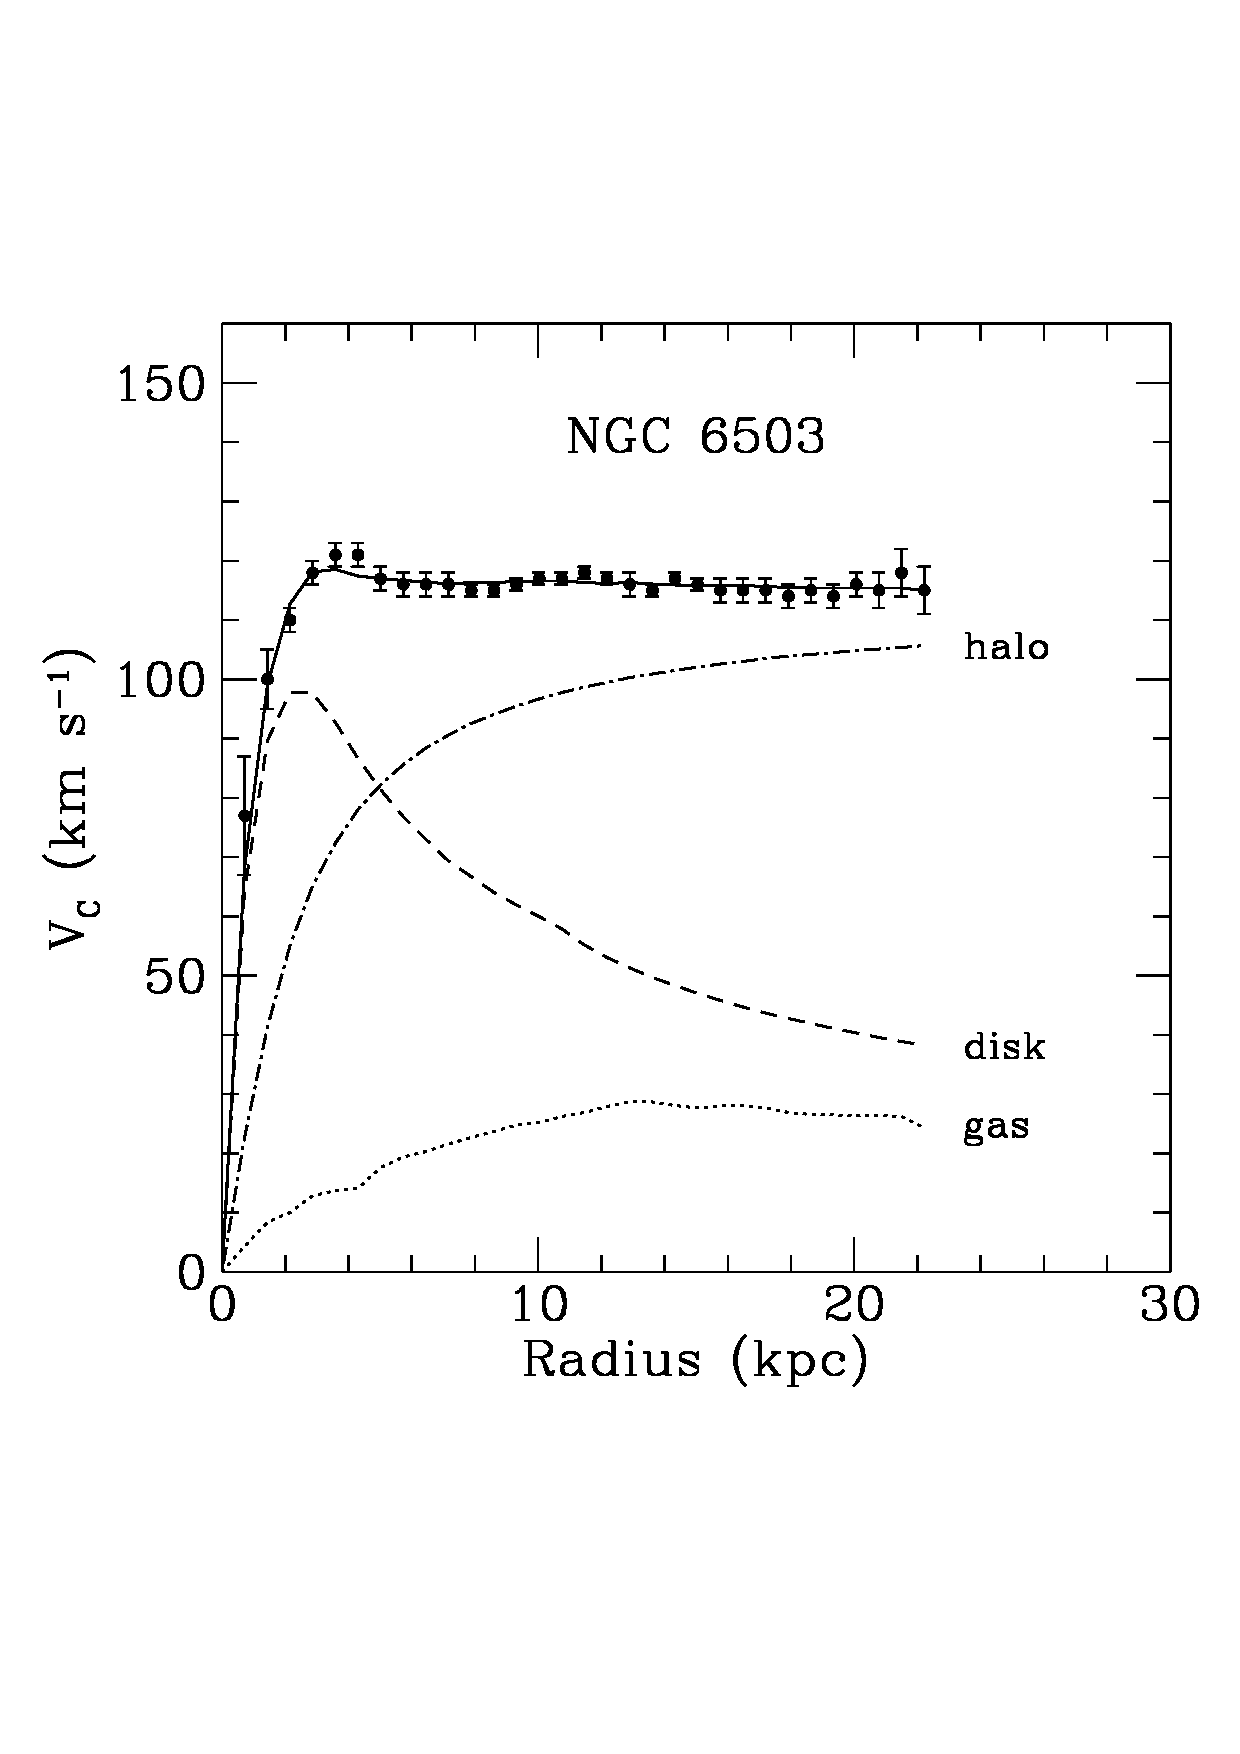
\includegraphics[width=0.4\textwidth]{imgs/Rotation}
    \caption{Rotation curve of the dwarf spiral galaxy NGC 6503 with the fitted halo, disc and gas distributions \cite{Begeman:1991iy}}
    \label{fg:RotationCurve}
\end{figure}
This rotation curve is shown in figure \ref{fg:RotationCurve} as an example. Newtonian circular orbits that should in this case at least be approximately obeyed demand 
\begin{equation}
v(r)=\sqrt{\frac{GM(r)}{r}}
\end{equation}
where $M(r)$ is the mass contained in a sphere of radius $r$ around the center of the galaxy. Without dark matter this is roughly constant beyond the optical disc such that the rotational velocity behaves like $v(r)\sim 1/\sqrt{r}$.
But the observation does not show this behaviour at all. Instead farther out the velocity becomes constant. This implies a halo of yet unaccounted mass with a density profile that falls off as $1/r^2$.

A better understanding of the distribution especially close to the center of this halo is an issue of ongoing research. \cite{Bertone:2004pz}

Another technique to deduce the distribution of mass in the universe that does not directly rely on the luminosity itself is gravitational lensing. Here a foreground galaxy or cluster bends space-time so that the light of a background object gets bend similar to an optical lens. Most impressive are constellations where the lensing object is circular and lines up with the background galaxy from the observers point of view. In this case the background galaxy gets distorted to a complete "Einstein ring", that appears with an angular "Einstein radius" 
\begin{equation}
\theta_E = \sqrt{\frac{4GM}{c^2}\frac{d_{LS}}{d_Ld_S}}
\end{equation}
where $M$ is the mass of the lensing object, $d_{LS}$ is the distance between the lens and source and $d_L (d_S)$ is the distance between the observer and the lens (source). Because the perfect alignment is rare, arcs rather than rings are observed. 
This fact was first used in the Abell 370 cluster to estimate the dark matter distribution and mass. One of the arcs used is shown in figure \ref{fg:abell}. 
\begin{figure}[ht]
  \centering
    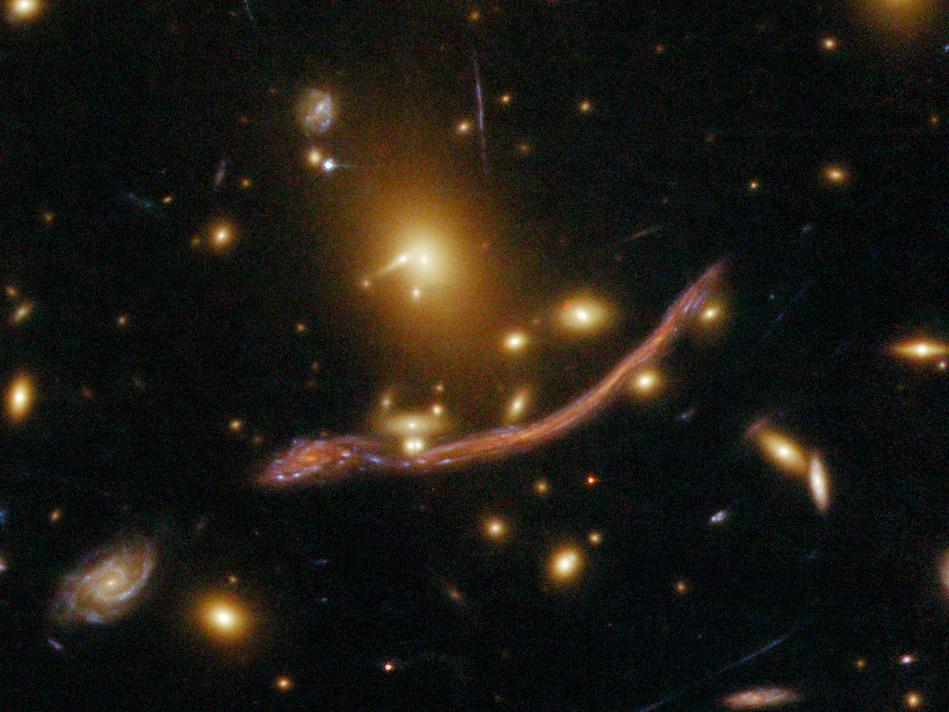
\includegraphics[width=0.4\textwidth]{imgs/large_web}
    \caption{Arc from gravitational lensing in Abell 370}
    \label{fg:abell}
\end{figure}
Comparing the necessary mass distribution for the lens and the optical distribution lead to two observations: Firstly again the luminous matter is far to light to account for the lensing and secondly the mass distribution also differs in position. 
This difference in position is most impressively shown in the bullet cluster shown in figure \ref{fg:bullet}. Here two clusters collided. During this collision the hot gas of both clusters interacted and is slowed. The dark matter component, lacking direct interaction is not slowed and continues largely its trajectory. This has also been used to falsify modified theories of gravitation. 
\begin{figure}[H]
  \centering
    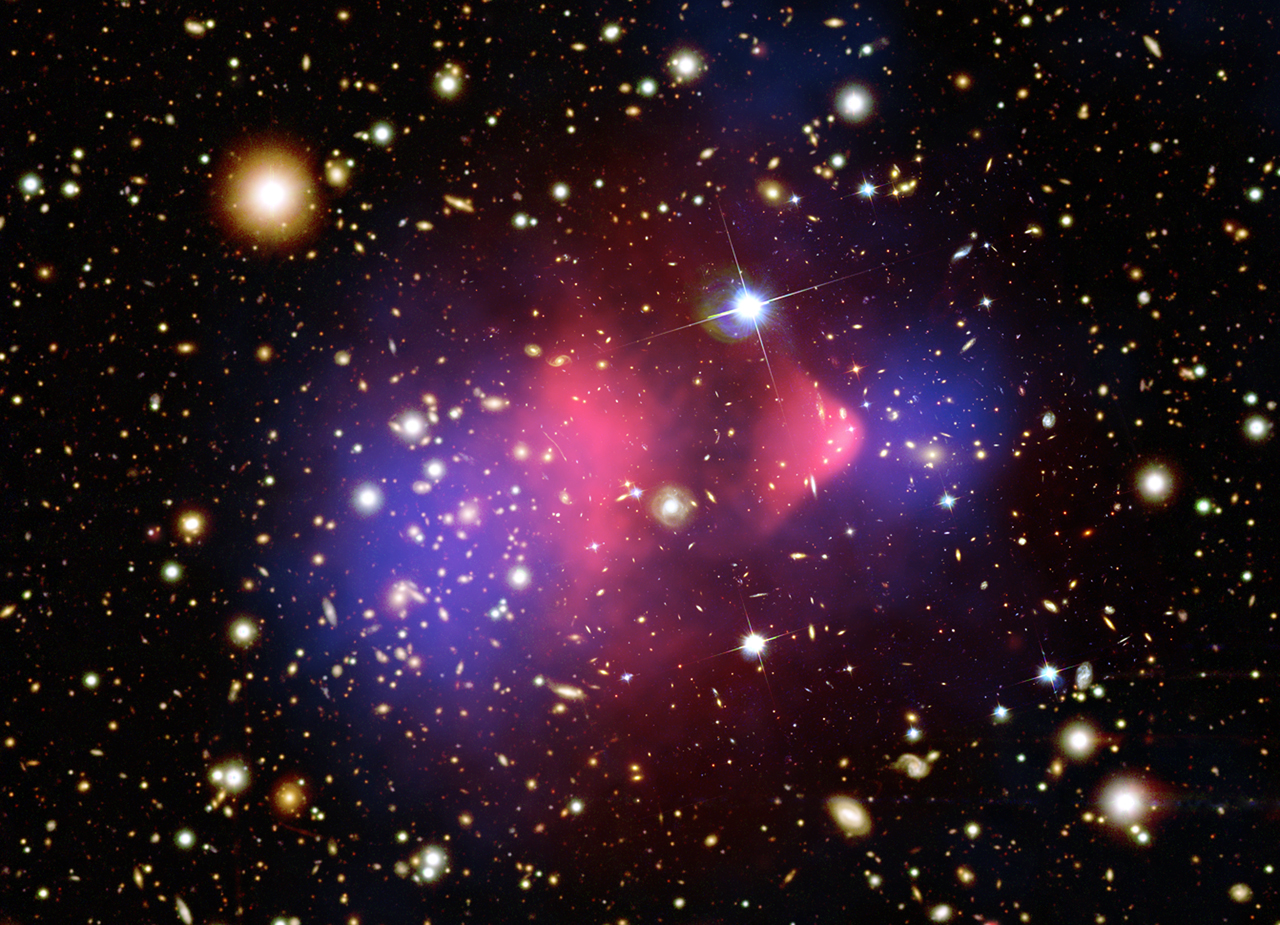
\includegraphics[width=0.4\textwidth]{imgs/bullet}
    \caption{Composite image of the galaxy cluster 1E 0657-556 with an X-ray image (red) and lensing mass distribution (blue) that do not coincide \cite{Massey:2010hh}}
    \label{fg:bullet}
\end{figure}

On much bigger scales the total amount of dark matter can be extracted from the Cosmic Microwave Background (CMB) in light of the recent survey by WMAP.
This has shown the CMB to be isotropic up to relative deviations of the order of $10^{-5}$. The remaining anisotropies can be used to constrain cosmological models.  Analysis of these distributions in the WMAP data results in
\begin{align}
\Omega_bh^2&=0.02264\pm0.00050\\
\Omega_Mh^2&=0.1364\pm0.0044
\end{align}
where $\Omega_b$ ($\Omega_M$) is the baryonic (matter) density relative to the critical density of the universe 
This further shows that the baryonic content is only responsible for a fraction of the entire matter content.


Since the large structure of the universe seems to strongly indicate the existence of dark matter, we still don't know what it is made of at the microscopic scale. All we know is that it interacts gravitationally but does not interact directly with light. 

The most strait forward remedy for this assumes dark matter to be made out of particles. Our job is then to develop models that at one hand explain the relic densities and on the other hand does not saturate existing bound of searches for new physics.

\section{Particle Dark Matter Candidates}
Dark matter candidates have to fulfil some conditions to be even worth considering. Since it should be present today, it either needs to be stable or its lifetime needs to be longer than the age of the Universe ($t_U=4\cdot 10^{17}s$).
Further it can't be electrically charged since it otherwise wouldn't be dark. And lastly it needs to reproduce the correct relic density
$\Omega_{DM}\sim 0.2$.
\paragraph{Axions}
Another interesting candidate is the the axion. 
Per se there is no reason for a CP-violating term to be absent in the theory. But the electric dipole moment of the neutron restricts \cite{Patrignani:2016xqp} an effective term like 
\begin{equation}
\mathcal{L}\supset -\Theta (\alpha_s/16\pi)F^{\mu\nu a}\epsilon_{\mu\nu\lambda\rho}F^{\lambda\rho a}
\end{equation}
to $|\Theta|\lesssim10^{-10}$. This can be explained by the introduction of the global Peccei-Quinn symmetry $U(1)_{PQ}$ that is subsequently spontaneously broken at the scale $f_A$. This cancels the aforementioned CP-violating term and introduces a pseudo Nambu-Goldstone boson -- the axion.
The axion-mass is then given by\cite{Bergstrom:2000pn}
\begin{equation}
m_A\approx 6\text{eV}\left(\frac{10^6\text{GeV}}{f_A}\right).
\end{equation}
The effective coupling constant of the axion to two photons is then proportional to $\alpha/f_A$. Thus the coupling and the mass of the axion can be simultaneously constrained.
Current bounds constrain the axion to be light ($\lesssim 10meV$). Even though the acceptable parameter strains gets smaller, there are still configurations where the axion might be the right dark matter candidate.

\paragraph{Neutrinos}
The standard model neutrinos are notoriously hard to detect and are already accounted for in the Standard Model. So at least that makes them seem to be good dark matter candidates. But since the total relic density can be estimated from the total mass of all three neutrino-generations to be $\Omega_\nu h^2 \lesssim 0.007$ , it will not suffice to account for all of the dark matter relic density.

\paragraph{SUSY}
To remedy the hierarchy problem of the Standard model one may introduce a new symmetry between bosons and fermions. Each particle has to have a super symmetric partner assigned that obeys the opposite statistics. If one extends the standard model to be super symmetric, the neutral $W$, $B$ and the neutral Higgs bosons (two different Higgs fields have to be introduced in SUSY) get fermionic superpartners that might mix to new mass eigenstates called neutralinos. To stop the proton from decaying, a new symmetry can be imposed -- the R-parity. If this is the case, the lightest of the neutralino will be stable and also serve as a dark matter candidate.

Since the super partners of neutrinos might acquire a large mass after SUSY-breaking these might also be seen as candidates. But the mass range that would result in the correct relic density is already ruled out by direct detection experiments searching for sneutrino-nucleon interactions.

\paragraph{Extra Dimensions}
Another somewhat different scenario are extra dimensions. There is no direct evidence, that the world we live in consists of more than three spacial and one temporal dimension. Nevertheless, extra dimensions are part of many beyond standard model theories. The idea that there might be more has received attention by Kaluza in his publication in 1921 that tried to unify gravity and electromagnetism in a five dimensional space-time so that Einstein's field equations yield general relativity and electromagnetism.
Modern QFT versions such as UED allow all fields to propagate in this extra dimension so that after compactification to for example a circle, their momentum-component gets quantised and result in so-called Kaluza-Klein states, that from the four dimensional point of view look like a tower of partner states with rising masses but same quantum numbers. A Kaluza-Klein-parity conservation then ensures, that the lightest state is stable and thus might serve as a dark matter candidate.